
\documentclass[12pt]{article}
%%%\documentclass[12pt,a4paper]{scrartcl}
\usepackage[left=3cm,right=3cm,top=2cm,bottom=2cm]{geometry} % page settings
\usepackage{lingmacros}
\usepackage{tree-dvips}
\usepackage[polish]{babel}
%%% fix for \lll
\let\babellll\lll
\let\lll\relax 
\usepackage[T1]{fontenc}


\usepackage{amssymb}
\usepackage{verbatim}
\usepackage{listings}
\usepackage{amsmath}
\usepackage{amsthm}
\usepackage[boxed]{algorithm2e}
\usepackage{float}
\usepackage{graphicx}

\renewcommand{\algorithmcfname}{Algorytm}
\SetKwInput{KwData}{\textbf{Dane}}
\SetKwInput{KwResult}{\textbf{Wynik}}
\renewcommand{\qedsymbol}{$\blacksquare$}

\title{Zadanie 3}
\author{Marko Golovko}
\date{\today}

\begin{document}
\maketitle

\section*{Definicja}
Rozkład Studenta z $n$ stopniami swobody jest rozkładem zmiennej losowej $T$ postaci:
	$$ T = \frac{U}{\sqrt{Z}}\sqrt{n}$$
gdzie:
\begin{itemize}
	\item $U$ jest zmienną losową mającą standardowy rozkład normalny $N(0,1)$,
	\item $Z$  jest zmienną losową o rozkładzie chi kwadrat o $n$ stopniach swobody,
	\item $U$ i $Z$ są niezależne.
\end{itemize}

\section*{Gęstość rozkładu. Obliczenia}
Z założenia znamy wżór na gęstość rozkładu normanlnego i rozkładu chi-kwadrat.  \\
Niech $U$ i $Z$ będą takie jak wyżej. Zmienna $Y = \sqrt{Z}$ ma rozkład chi o $n$ 
stopniach swobody, a więc $Y$ wyraża się wzorem 
	
$$ f_{Y}(y)=\frac{2^{1-\frac{n}{2}}y^{n-1}e^{-\frac{y^{2}}{2}}}{\Gamma(\frac{n}{2})} $$
Rozważmy zmienną 
$$ X = \frac{1}{\sqrt{n}}Y$$
Policzymy rozkład prawdopodobieństwa zmiennej X. Korzystamy z własności rozkładów prawdopodobieństwa. \\
Jeżeli $ g:{\mathbb {R_{+}} }\rightarrow {\mathbb {R_{+}}}$ funkcja monotonczna, wtedy rozkład prawdopodobieństwa jest

 $$ f_{X}(x)=f_{Y}(g^{-1}(x))|{\frac {d}{dx}} (g^{-1}(x))| = f_{Y}(g^{-1}(x))|{\frac {d}{dx}}(y)| = f_{Y}(y)|\frac {dy}{dx}| . $$
 $$ |\frac {dy}{dx}| = \sqrt{n}$$
 $$ f_{X}(x) = f_{Y}(\sqrt{n}x)|\frac {dy}{dx}| = 
 \frac{2^{1-\frac{n}{2}}(\sqrt{n}x)^{n-1}e^{-\frac{(\sqrt{n}x)^{2}}{2}}}{\Gamma(\frac{n}{2})}\sqrt{n} = 
 \frac{2^{1-\frac{n}{2}}n^{\frac{n}{2}}x^{n-1}e^{-\frac{n}{2}x^{2}}}{\Gamma(\frac{n}{2})}$$
	
Zmienna $T$ ma zatem rozkład $\frac{U}{X}$. Jej gęstość jest więc postaci rozkładu ilorazu. \\
Aby obliczyć iloraz $T = \frac{U}{X}$ dwóch niezależnych zmiennych losowych $U$ i $X$, 
zdefiniujemy następującą transformację:
$$T = \frac{U}{X}$$
$$W = X$$
Więc wspólne prawdopodobieństwo $p(t,w)$ może być policzone zamianą zmiennych z $U,X$ do $T,W$, 
i $T$ można uzyskać przez rozkład brzegowy W z wspólnego rozkładu prawdopodobieństwa. \\
Odwrotna transformacja

$$U = TW$$
$$X = W$$
Jacobian $J(U,X\mid T,W)$ naszego przekzstalcenia wyraża się macierzą
$$\begin{vmatrix}{\frac {du}{dt}}&{\frac {du}{dw}}\\
{\frac {dx}{dt}}&{\frac {dx}{dw}}\end{vmatrix}=
{\begin{vmatrix}w&t\\0&1\end{vmatrix}}=|w|. $$
A zatem
$$ p(t,w)=p(u,x)J(u,x\mid t,w)=
p(u)p(x)J(u,x\mid t,w)=p_{U}(tw)p_{X}(w)|w|.  $$
I $T$ można uzyskać przez rozkład brzegowy W
$$p(t)=\int _{-\infty }^{\infty }p_{U}(tw)p_{X}(w)|w|dw $$
Więc 
$$ f_{T}(t)=\int _{-\infty }^{\infty }f_{U}(tw)f_{X}(w)|w|dw =
   \int _{0 }^{\infty }wf_{U}(tw)f_{X}(w)dw = $$
  $$ \int _{0 }^{\infty }w \frac{1}{\sqrt{2\pi}}e^{-\frac{(tw)^2}{2}} 
   \frac{2^{1-\frac{n}{2}}n^{\frac{n}{2}}w^{n-1}e^{-\frac{n}{2}w^{2}}}{\Gamma(\frac{n}{2})}dw  =  
   \frac{2^{1-\frac{n}{2}}n^{\frac{n}{2}}}{\sqrt{2\pi}\Gamma(\frac{n}{2})}
   \int _{0 }^{\infty } w^{n}e^{-\frac{1}{2}(n+t^{2})w^{2}}dw $$
Niech $m = x^{2}$ $(dm=dx(x^{2})=2xdx)$. Wówczas powyższa całka przyjmuje postać
$$ \int _{0 }^{\infty } w^{n}e^{-\frac{1}{2}(n+t^{2})m}\frac{dm}{2x}=
	\frac{1}{2}\int _{0 }^{\infty }m^{\frac{n-1}{2}}e^{-\frac{1}{2}(n+t^{2})m}dm $$
Gęstość $f(m;k;\theta)$ rozkładu Gamma wyraża się wzorem

$$ f(m;k;\theta)=\frac{m^{k-1}e^{-\frac{m}{\theta}}}{\theta^{k}\Gamma(k)} $$
Oznacza to, że
$$ k-1 = \frac{n-1}{2} \Rightarrow k^* = \frac{n+1}{2}, \quad 
\frac{1}{\theta} = \frac{1}{2}(n+t^2)\Rightarrow\theta^*=\frac{2}{(n+t^2)},$$

jeżeli korzystamy z własności mediany Gamma rozkładu
$$ \frac{1}{\Gamma(k)\theta^k}\int _{0}^{v} x^{k-1}e^{-x/\theta}dx = \frac{1}{2} $$

stąd powyższa całka 
$$ \int _{0 }^{\infty } m^{k^*-1}e^{-\frac{m}{\theta^*}} = 
	\frac{1}{2}\Gamma(k^*)(\theta^*)^{k^*} = 
	\frac{1}{2}(\frac{2}{n+t^2})^\frac{n+1}{2}\Gamma(\frac{n+1}{2}) =$$
$$ 2^{\frac{n-1}{2}}n^{-\frac{n+1}{2}}\Gamma(\frac{n+1}{2})(1+\frac{t^2}{n})^{-\frac{1}{2}(n+1)}$$
Ostatecznie
$$ f_{T}(t)= \frac{2^{1-\frac{n}{2}}n^{\frac{n}{2}}}{\sqrt{2\pi}\Gamma(\frac{n}{2})}
2^{\frac{n-1}{2}}n^{-\frac{n+1}{2}}\Gamma(\frac{n+1}{2})(1+\frac{t^2}{n})^{-\frac{1}{2}(n+1)}= 
\frac{\Gamma((n+1)/2)}{\sqrt{n\pi}\Gamma(n/2)}(1+\frac{t^2}{n})^{-\frac{1}{2}(n+1)} $$
\section*{Dystrybuanta.  Numeryczna wartość}

$$F(x) = \int_{-\infty}^{x}f(t)dt =
 \int_{-\infty}^{x} \frac{\Gamma((n+1)/2)}{\sqrt{n\pi}\Gamma(n/2)}(1+\frac{t^2}{n})^{-\frac{1}{2}(n+1)}dx = 
  \frac{\Gamma((n+1)/2)}{\sqrt{n\pi}\Gamma(n/2)}\int_{-\infty}^{x} (1+\frac{t^2}{n})^{-\frac{1}{2}(n+1)}dx$$
  Rozbijamy zadanie na dwie części.
\subsection*{Gamma funkjca}
Dla liczb naturalnych
$$ \Gamma(n)=(n-1)!$$
W naszym zadaniu oprócz liczb naturalnych będziemy liczyli dla  $\mathbb {Q_{+}}$. Więc potrzebujemy takie wzory
$$ \Gamma (n+1) = n\Gamma(n) $$
$$ \Gamma (1-n)\Gamma(n) = \frac{\pi}{sin(\pi n)} $$
Dla $1<n<2$ będziemy aproksymować z pomocą wzoru
$$ \Gamma(n) \approx 1 + \frac{P_{0}^8(x)}{P_{1}^8(x)}, \quad
x = n-1; $$
gdzie 
	$$P_{0}^8(x)= \sum_{k=1}^{8}a_{k}x^k $$
	$$P_{1}^8(x)= \sum_{k=1}^{8}b_{k}x^{k-1}+x^8 $$
Wartości $a_k$ i $b_k$ bierzemy z tablicy. Wartości tablicy i obliczenia Gamma funkcji znajdują się w pliku gamma.jl, żeby nie zmniejszać czytelność, nie pokazuję zawartości tego pliku.
\subsection*{Funkcja podcałkowa}
$$ \int_{-\infty}^{x} (1+\frac{t^2}{n})^{-\frac{1}{2}(n+1)}dx $$
Jest symetryczna względem osi 0Y. Więc możemy ją przekształcić.
$$ 2\int_{0}^{x} (1+\frac{t^2}{n})^{-\frac{1}{2}(n+1)}dx $$
Liczymy wartość całki za pomocą funkcji Romberga znajdującą w pliku romberg.jl
\subsection*{Numeryczna wartość}
Dla przykładu wybrałem n = [1,10,30] i zrobiłem trzy wykresy.
Obliczenia znajdują się w pliku t-studentCNF.jl
\begin{figure}[hbt!]
 \centering
 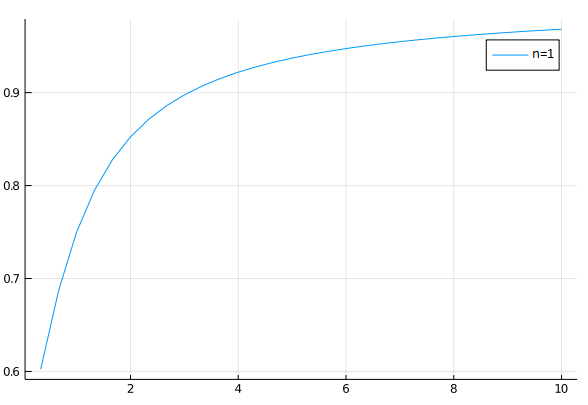
\includegraphics{n1s}
\end{figure}
\begin{figure}[hbt!]
 \centering
 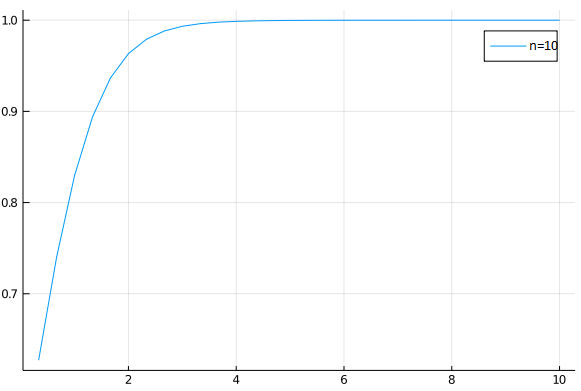
\includegraphics{n10s}
 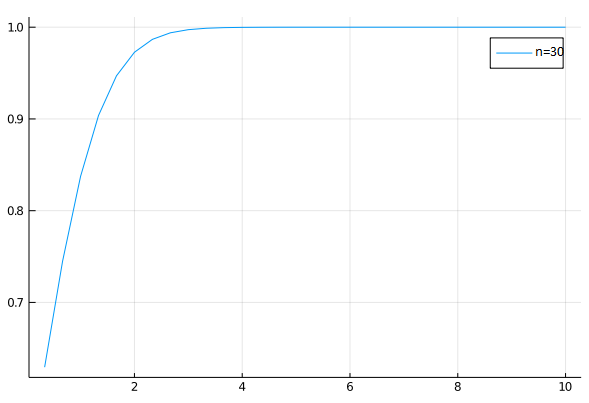
\includegraphics{n30}
\end{figure}








\end{document}